\chapter{Конструкторская часть}

В данном разделе будет рассмотрена схема вышеизложенного алгоритма.

\section{Разработка алгоритмов}

На рисунках \ref{img:alg1} -- \ref{img:alg2} представлен алгоритм удаления элементов, больших $k$, где $k\in [1,Q]$ ($Q$ --- вход).

\begin{figure}[H]
	\begin{center}
		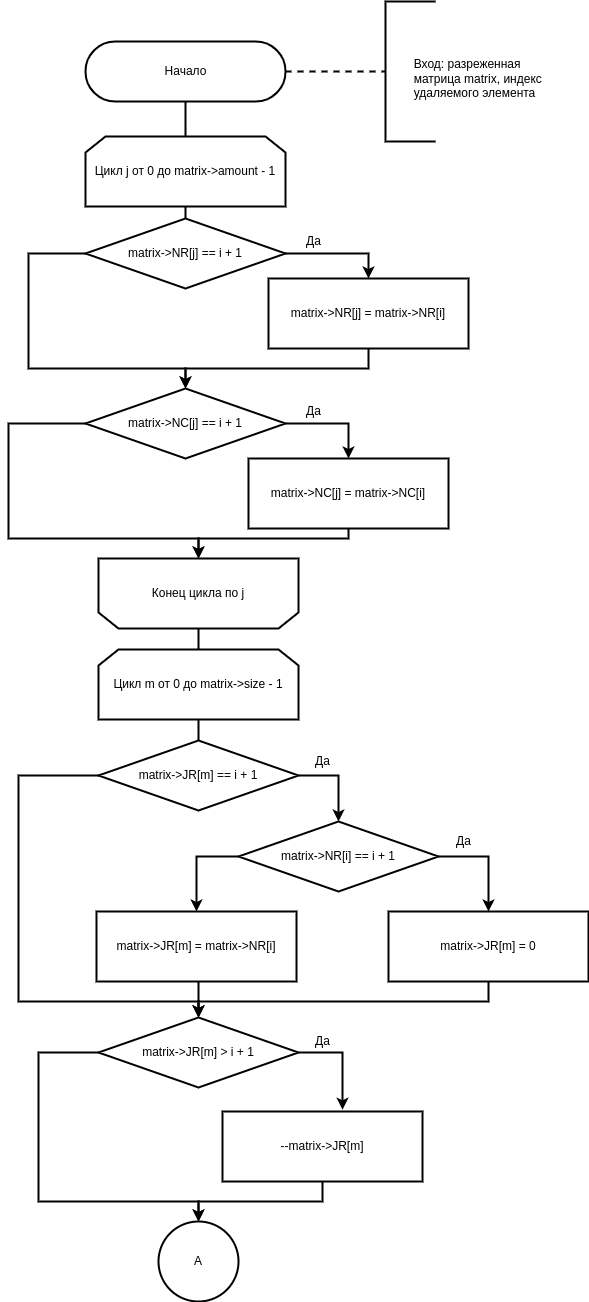
\includegraphics[scale=0.51]{img/alg1.png}
	\end{center}
	\captionsetup{justification=centering}
	\caption{Схема алгоритма удаления элемента (1 часть)}
	\label{img:alg1}
\end{figure}

\begin{figure}[H]
	\begin{center}
		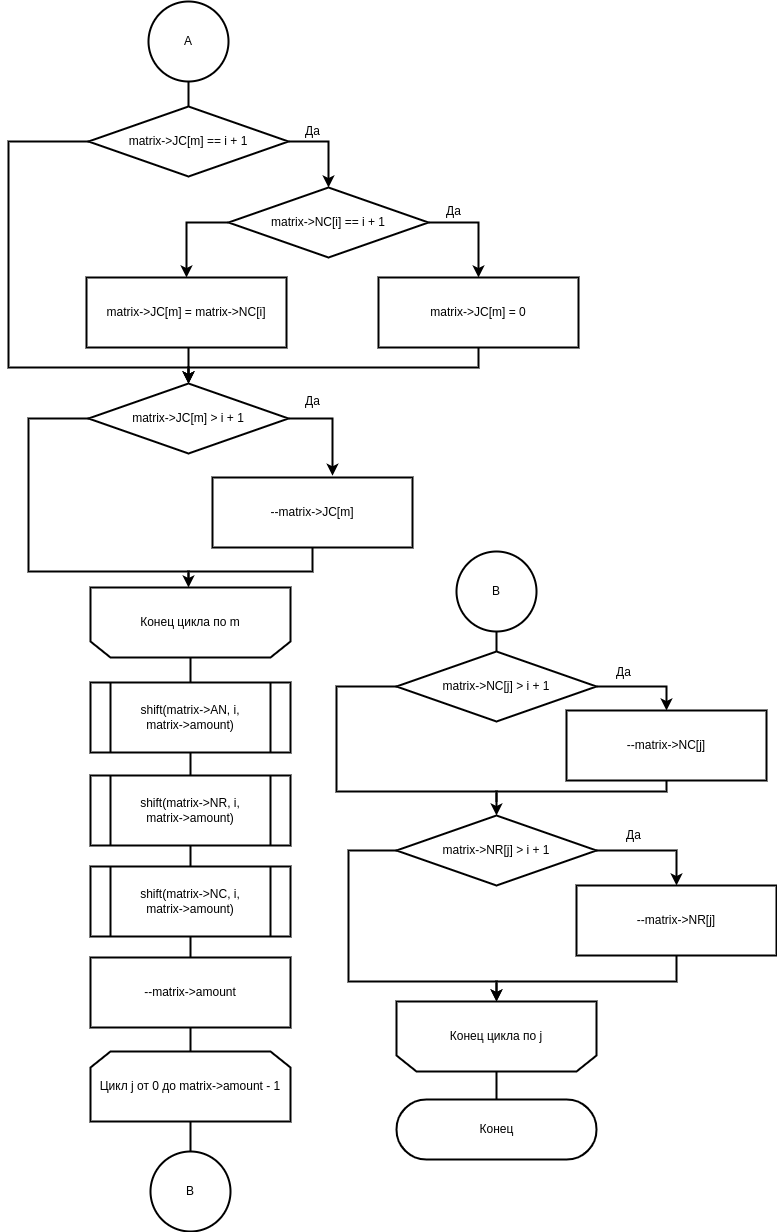
\includegraphics[scale=0.51]{img/alg2.png}
	\end{center}
	\captionsetup{justification=centering}
	\caption{Схема алгоритма удаления элемента (2 часть)}
	\label{img:alg2}
\end{figure}

На рисунке \ref{img:sequential} представлен последовательный алгоритм получения из верхнетреугольной матрицы набора матриц, из которых исключены значения, большие $k$, где $k\in [1,Q]$ ($Q$ --- вход).

\begin{figure}[H]
	\begin{center}
		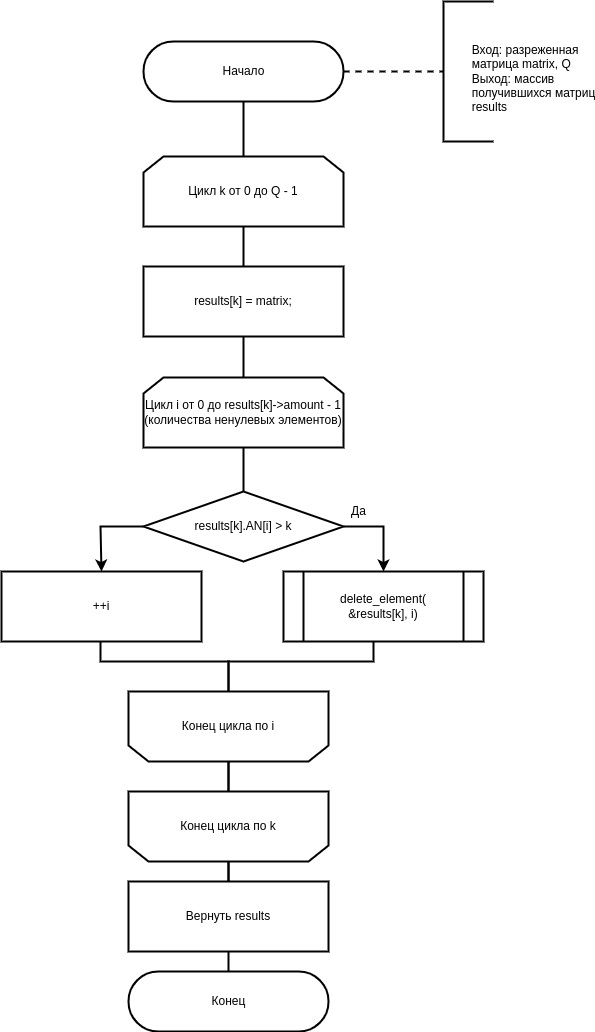
\includegraphics[scale=0.6]{img/sequential.png}
	\end{center}
	\captionsetup{justification=centering}
	\caption{Схема последовательного алгоритма}
	\label{img:sequential}
\end{figure}

На рисунке \ref{img:multithreading} представлен алгоритм запуска и ожидания потоков.

\begin{figure}[H]
	\begin{center}
		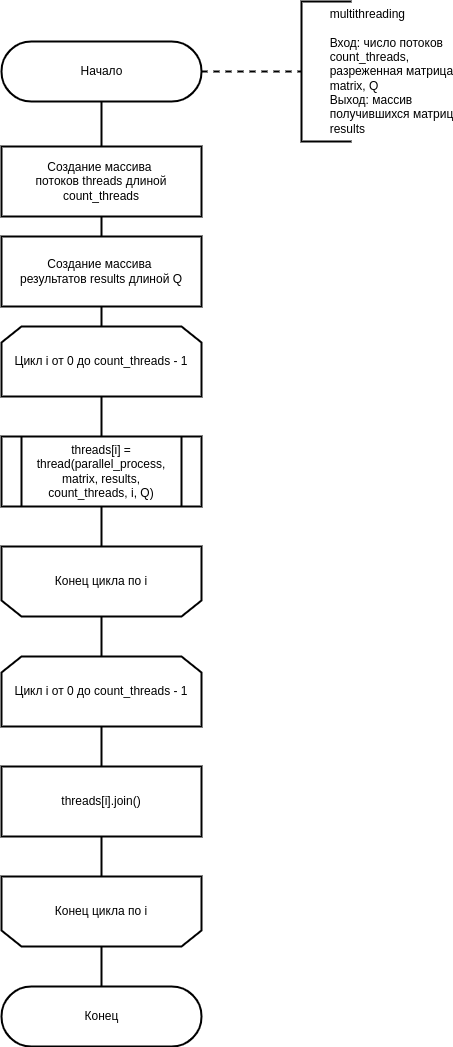
\includegraphics[scale=0.6]{img/multithreading.png}
	\end{center}
	\captionsetup{justification=centering}
	\caption{Схема запуска и одидания потоков}
	\label{img:multithreading}
\end{figure}

На рисунке \ref{img:parallel} представлен параллельный алгоритм получения из верхнетреугольной матрицы набора матриц, из которых исключены значения, большие $k$, где $k\in [1,Q]$ ($Q$ --- вход).

\begin{figure}[H]
	\begin{center}
		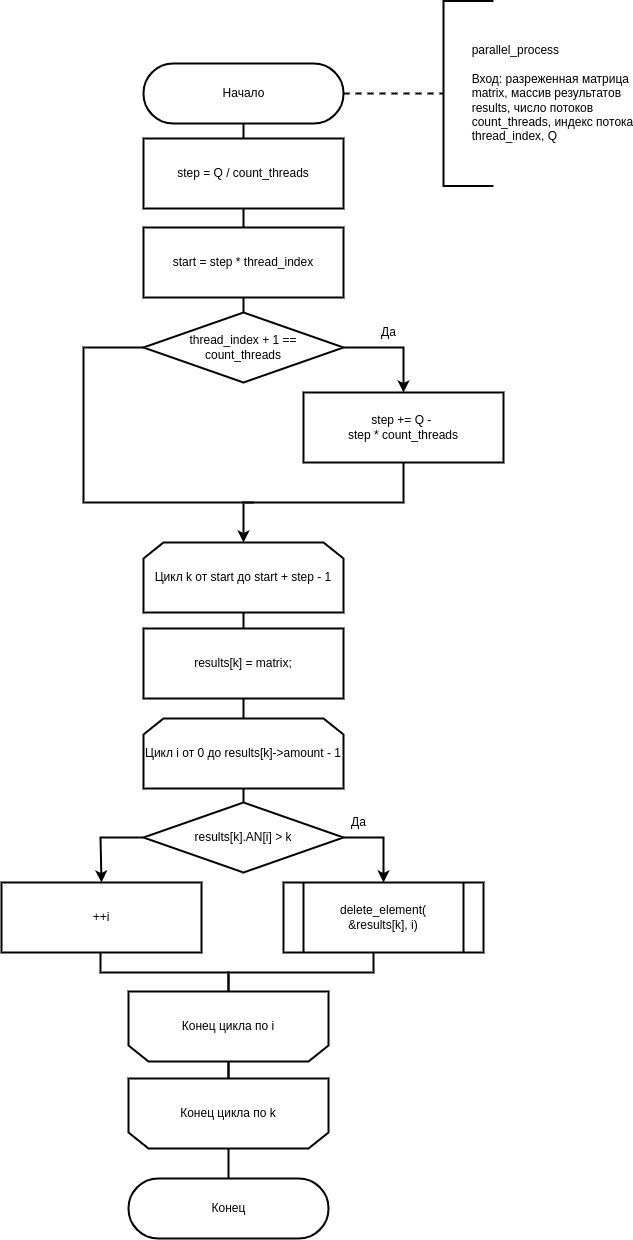
\includegraphics[scale=0.52]{img/parallel.png}
	\end{center}
	\captionsetup{justification=centering}
	\caption{Схема параллельного алгоритма}
	\label{img:parallel}
\end{figure}

\section*{Вывод}

На основе теоретических данных, полученных из аналитического раздела,
была построена схема требуемого алгоритма.
